\documentclass[a4paper]{article}

%use the english line for english reports
%usepackage[english]{babel}
\usepackage[portuguese]{babel}
\usepackage[utf8]{inputenc}
\usepackage{indentfirst}
\usepackage{graphicx}
\usepackage{verbatim}  

\usepackage[T1]{fontenc}
\usepackage{listings}
\usepackage{xcolor}

\usepackage{inconsolata}
\lstset{
    language=Prolog, %% Troque para PHP, C, Java, etc... bash é o padrão
    basicstyle=\ttfamily\small,
    numberstyle=\footnotesize,
    numbers=left,
    backgroundcolor=\color{gray!10},
    frame=single,
    tabsize=2,
    rulecolor=\color{black!30},
    title=\lstname,
    escapeinside={\%*}{*)},
    breaklines=true,
    breakatwhitespace=true,
    framextopmargin=2pt,
    framexbottommargin=2pt,
    extendedchars=false,
    inputencoding=utf8
}


\begin{document}

\setlength{\textwidth}{16cm}
\setlength{\textheight}{22cm}

\title{\Huge\textbf{Symple}\linebreak\linebreak\linebreak
\Large\textbf{Relatório Final}\linebreak\linebreak

\includegraphics[height=6cm, width=7cm]{feup.pdf}\linebreak \linebreak
\Large{Mestrado Integrado em Engenharia Informática e Computação} \linebreak \linebreak
\Large{Programação em Lógica}\linebreak
}

\author{\textbf{Grupo 41:}\\ André Duarte - 201100766 \\ João Carlos Santos - 201106760 \\\linebreak\linebreak \\
 \\ Faculdade de Engenharia da Universidade do Porto \\ Rua Roberto Frias, s\/n, 4200-465 Porto, Portugal \linebreak\linebreak\linebreak
\linebreak\linebreak\vspace{1cm}}
%\date{Junho de 2007}
\maketitle
\thispagestyle{empty}

%************************************************************************************************
%************************************************************************************************

\newpage

\section*{Resumo}
O objectivo do trabalho é implementar o jogo de tabuleiro Symple, recorrendo à linguagem Prolog e ao sistema de desenvolvimento SICStus Prolog,  no contexto da unidade curricular de Programação Logica.
Symple é um jogo de estratégia para duas pessoas publicado em 2010 por Christian Freeling e Benedikt Rosenau em que os jogadores competem por ocupar o maior número de quadrículas com o menor número de grupos de peças isolados. 

\newpage

\tableofcontents

%************************************************************************************************
%************************************************************************************************

%*************************************************************************************************
%************************************************************************************************

\newpage

\section{Introdução}
Entende-se por objectivo principal do projecto adquirir conhecimentos e sensibilidade na área de Programação em Lógica (utilizando neste caso Prolog) e desta forma desenvolver novas formas de raciocínio que de outra forma não seriam apreendidas. Por outro lado também se pretende obter algum tacto no desenvolvimento de jogos.

Este jogo apresenta características bastante peculiares, o que resulta num fluxo de jogo bastante original. Apesar de aparentar ser bastante simples, o jogo apresenta um conjunto de regras complexo e baseia-se primariamente em princípios matemáticos. O jogador tem que determinar a forma mais eficiente de multiplicar o seu número de peças tendo em conta as limitações a cada instante do jogo levando a estratégias permanentemente dinâmicas.

Por outro lado, visto que o tamanho do tabuleiro é variável os jogos podem ter durações variadíssimas dependendo do tempo disponível aos jogadores (por exemplo, um tabuleiro de 9x9 demorará aproximadamente três vezes mais tempo a acabar).

%*************************************************************************************************
%************************************************************************************************

\section{O Jogo Symple}

Symple é um jogo de estrategia abstrato em que dois jogadores competem para conseguir ocupar o maior número de casas do tabuleiro com o menor número de grupos possível.
As jogadas são feitas alternadamente entre dois jogadores, de cor Branca e Preta. O jogador 1 é o primeiro a jogar e joga com as peças brancas. O jogador 2 joga com as peças pretas.
No seu turno, um jogador pode escolher entre as seguintes jogadas:

\begin{enumerate}
\item Colocar uma peça no tabuleiro num sítio sem contacto com as outras peças, desta forma criando um novo grupo de peças.

\item Fazer crescer todos os grupos com uma peça. Peças que toquem em dois grupos contam como fazendo crescer ambos os grupos. No entanto, se dois grupos crescem em uma pedra e apenas as novas peças estão em contacto, a jogada e legal.
\end{enumerate}

Para equilibrar o jogo existe uma regra extra: se nenhum jogador tiver crescido os seus grupos, o jogador 2, que joga com as peças pretas, pode, na mesma jogada, crescer todos os seus grupos e criar um novo grupo.

O jogo termina quando o tabuleiro é preenchido. A pontuação é determinada pelo número de pedras que cada jogador tem no tabuleiro menos 'P' vezes o numero de grupos que o jogador tem, em que 'P' e um numero par maior ou igual a 4.
Ganha o jogador com a maior pontuação, que pode até nem ser o jogador com mais peças no tabuleiro! 

Com uma penalidade par (P vezes o número de grupos do jogador) e um tamanho de tabuleiro ímpar não são possíveis empates.

%*************************************************************************************************
%************************************************************************************************

\section{Arquitectura do Sistema}
% Descrever em linhas gerais o sistema e os módulos conceptuais que o constituem. Deve ser abordada a comunicação com o visualizador a desenvolver em LAIG, mesmo que ainda não esteja implementada.

O Sistema foi divido nas suas componentes de jogo, inteligência artifical e utilidades.

A componente de jogo consiste na interface com o utilizador e funções principais de jogadas.

A componente da inteligência artificial simula um utilizador, permitindo ainda a criação de diversos níveis diferentes muito facilmente, visto termos separado a escolha da jogada com o movimento em si.

Temos ainda a componente utilidades aglomera funções úteis aos últimos dois componentes descritos.

Estes componentes são ligados através de um componente principal que carrega e inicia tudo o que é necessário para dar ínicio ao jogo.

Quando for desenvolvida a interface gráfica esta vai comunicar através de sockets com a componente de jogo, enviando-lhe pedidos e reavendo informação.

%*************************************************************************************************
%************************************************************************************************

\section{Lógica do Jogo}
%Descrever o projeto e implementação do módulo Prolog, incluindo a forma de representação do estado do tabuleiro, execução de movimentos, verificação do cumprimento das regras do jogo, determinação do final do jogo e cálculo das jogadas a realizar pelo computador utilizando diversos níveis de jogo. Sugere-se a estruturação desta secção da seguinte forma:

%*************************************************************************************************
%************************************************************************************************

\subsection{Representação do Estado do Jogo} 
Visto tratar-se de um jogo com tabuleiro quadrado, representamos-o numa lista de listas dinâmica.

Logicamente as listas apresentam-se da seguinte forma:

\begin{itemize}

\item B = [ L1, L2, L3, ..., LN ], em que B simboliza o tabuleiro (board) e cada L representa uma linha do tabuleiro
\item L = [ C1, C2, C3, ..., LN ], em que cada C representa uma coluna do tabuleiro
\item C = [ [J1, G1], [J1, G2], [J2, G1], ..., [J2, G2] ], em que para cada posição existe uma lista que representa a peça, com o jogador e o número do seu grupo ao qual a peça pertence: J1 representa o jogador 1, J2 o jogador 2, G1 o grupo 1, etc... Dois jogadores podem ter o mesmo número a identificar o grupo da peça, sendo que os grupos de cada jogador são processados de forma independente.

\end{itemize}
%*************************************************************************************************
%************************************************************************************************

\subsection{Visualização do Estado do Jogo} 
\textit{printBoard(+Tabuleiro).}

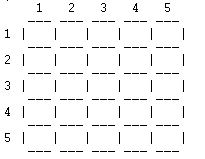
\includegraphics{prologMap.JPG}

%*************************************************************************************************
%************************************************************************************************

\subsection{Validação de Jogadas} É feita imediatamente e automaticamente antes da execução da jogada. Através de diversas funções:

\textit{checkPlace(+Tabuleiro, +Coluna, +Linha).}

\textit{checkNotAdjacent(+Tabuleiro, +Coluna, +Linha, +Jogador).}

\textit{checkNotExpanded(+GruposExpandidos, +Grupos).}

\textit{checkGrow(+Grupos).}


Exemplo de Jogada Create

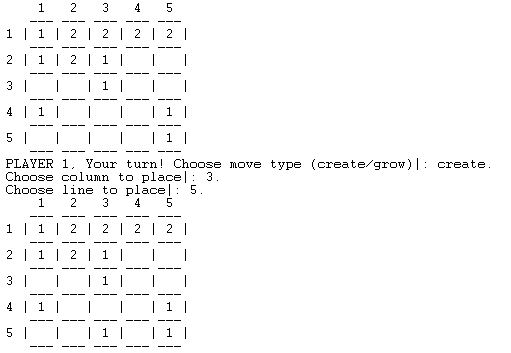
\includegraphics{prologCreate.JPG}

Exemplo de Jogada Grow

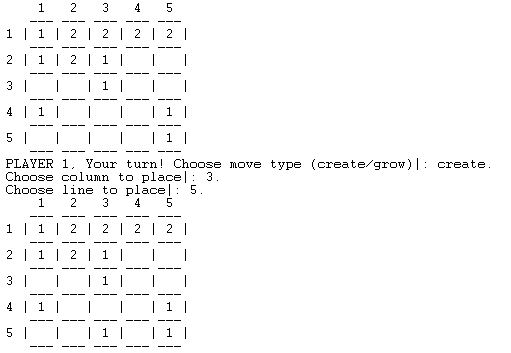
\includegraphics{prologCreate.JPG}

%*************************************************************************************************
%************************************************************************************************

\subsection{Execução de Jogadas} A execução de jogadas é diferente caso seja um Jogador ou a AI.
Se for um jogador são invocadas as seguintes funções:

\textit{manualMove(+Jogador, +Tabuleiro, -NovoTabuleiro, +Jogada).}

\textit{pieceGrow(+Tabuleiro, -NovoTabuleiro, +Jogador, +GruposDoJogador, -NovosGruposDoJogador, +Coluna, +Linha).}

\textit{pieceCreate(+Tabuleiro, -NovoTabuleiro, +Jogador, +Coluna, +Linha).}


 
%*************************************************************************************************
%************************************************************************************************

\subsection{Lista de Jogadas Válidas} Usamos listas de jogadas válidas quando trabalhamos com a AI e para tal desenvolvemos as seguintes funções:

\textit{getPossibleCreatePieces(+Tabuleiro, +Jogador, --Resultado).}

\textit{getPossibleGrowPieces(+Tabuleiro, +Jogador, +GruposExpandidos, -Resultado).}

\textit{checkPointGetPossibleGrowPieces(+Tabuleiro, +Jogador, +Colunas, +Linhas, -GruposExpandidos).}

%*************************************************************************************************
%************************************************************************************************

\subsection{Avaliação do Tabuleiro} Existem várias funções que avaliam o estado do tabuleiro de modo a determinar se uma jogada é ou não válida:

\textit{checkNotAdjacent(+Tabuleiro, +Coluna, +Linha, +Jogador)).}

\textit{checkPlace(+Tabuleiro, +Coluna, +Linha) .}

\textit{checkGrow(+GruposDoJogador).}

\textit{checkNotExpanded(+GruposExpandidos, +Grupo).}

%*************************************************************************************************
%************************************************************************************************

\subsection{Final do Jogo} A verificação do fim do jogo é feita pela seguinte função:

\textit{checkGameEnd(+Tabuleiro)}

Esta é chamada antes de cada jogada e caso retorne true é mostrado o resultado.

A pontuação final de cada jogador é calculada pela seguinte função:

\textit{calculatePoints(+Tabuleiro, -PontosDoJogador1, -PontosDoJogador2).}
%*************************************************************************************************
%************************************************************************************************

\subsection{Jogada do Computador} Escolha da jogada a efetuar pelo computador, dependendo do nível de dificuldade. Por exemplo: \textit{aiMove(+Tabuleiro, +NovoTabuleiro, +Dificuldade (1 ou 2), +Jogador, +NumeroDaJogada).}


%*************************************************************************************************
%************************************************************************************************

\section{Interface com o Utilizador}
Durante todo o jogo o(s) utilizador(es) não precisa(m) de saber nenhum predicado, sendo-lhe(s) pedida apenas informação relacionada com o jogo.

Logo de início é pedido o tamanho do tabuleiro e o Modo de Jogo, que pode ser uma de três opções:
\begin{enumerate}
\item Jogador Humano vs. Jogador Humano
\item Jogador Humano vs. AI Fácil
\item Jogador Humano vs. AI Difícil
\end{enumerate}

Logo a seguir é apresentada ao jogador 1 o tabuleiro e a seguinte mensagem: "PLAYER 1, Your turn! Choose move type (create/grow): "

A esta mensagem o jogador responde com "create" ou "grow", obviamente. Caso responda de forma errada é-lhe apresentada a mensagem "Invalid Move" e volta a ter que escolher uma jogada.

Iniciada a jogada, pergunta as posições de cada peça e em caso de jogada inválida pergunta novamente o tipo de jogada que pretende fazer. De forma a permitir ao jogador trocar o tipo de jogada em caso de engano.

Acabada a jogada é apresentado o tabuleiro novamente, com as novas colocações.

%*************************************************************************************************
%************************************************************************************************

\section{Conclusões e Perspectivas de Desenvolvimento}
Com este trabalho concluímos que o Prolog é uma linguagem de programação interessante e que foi desafiador fazer um jogo num tipo de programação diferente do que estamos habituados.

O resultado foi animador.

%*************************************************************************************************
%************************************************************************************************

\clearpage
\addcontentsline{toc}{section}{Bibliografia}
\renewcommand\refname{Bibliografia}

\begin{thebibliography}{9}

\bibitem{BGG}
  Board Game Geek,
  \emph{Symple}.
  http://boardgamegeek.com/boardgame/106341/symple,
  2010. Online em Novembro de 2013.
  
\bibitem{MS}
  MindSports,
  \emph{Symple}.
  http://www.mindsports.nl/index.php/arena/symple,
  2010. Online em Novembro de 2013.

\end{thebibliography}

\newpage
\appendix
\section{Anexo}
%\begin{lstlisting}
\lstinputlisting{main.pl}
\lstinputlisting{ai.pl}
\lstinputlisting{board.pl}
\lstinputlisting{symple.pl}
\lstinputlisting{utilities.pl}
%\end{lstlisting}

\end{document}